\begin{problem}{Fermat's Last Theorem}{Inn}{Út}{~}{~}

	\begin{wrapfigure}{r}{0.27\textwidth}
		\vspace{-25pt}
		\begin{center}
			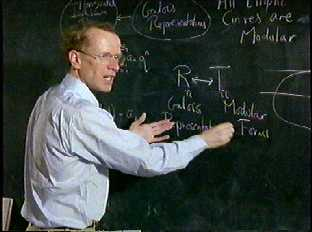
\includegraphics[scale=0.5]{../FermatsLastTheorem/Wiles5.jpg}
		\end{center}
		\vspace{-50pt}
	\end{wrapfigure}

	Pierre de Fermat er franskur stærðfræðingur sem uppi var á 17.\ öld. Þekktastur er hann fyrir eftirfarandi tilgátu:

	\begin{center}
		\textit{Ekki eru til neinar pósitífar heiltölur $a$, $b$ og $c$ sem uppfylla\\ jöfnuna $a^n + b^n = c^n$ þegar $n$ er heiltala stærri en $2$.}
	\end{center}

	Fermat skrifaði þessa tilgátu í spássíu bókar sem hann var að lesa, og sagðist hafa sönnun fyrir tilgátunni, en hún væri of löng til að komast fyrir á spássíunni. Margir stærðfræðingar reyndu að sanna tilgátuna eftir þetta, en það var ekki fyrr en rúmlega 300 árum síðar að breski stærðfræðingurinn Andrew Wiles kom loksins með sönnun. Tilgátan reyndist því vera sönn, og er nú kölluð "`síðasta setning Fermats."'

	\Input

		Á fyrstu línu er heiltalan $1 \leq T \leq 100$, sem táknar fjölda prófunartilvika sem fylgja. Hvert prófunartilvik samanstendur af einni línu með heiltölunni $2 < n < 10^{100}$.

	\Output

		Fyrir hvert prófunartilvik á að skrifa út allar pósitífar heiltölur $a$, $b$ og $c$ sem uppfylla jöfnuna $a^n + b^n = c^n$. Skrifa á út eina lausn á línu á forminu "`\texttt{$a$ $b$ $c$}"'. Ekki skiptir máli í hvaða röð lausnirnar eru skrifaðar út. Ef það eru ekki neinar lausnir, þá á að skrifa út eina línu á forminu "`\texttt{no solutions when n = $n$}"'.

	\Examples

		\begin{example}
			\exmp{
2
3
42
			}{
no solutions when n = 3
no solutions when n = 42
}%
		\end{example}

\end{problem}